\documentclass[12pt, a4paper]{article}
\title{Туннелирование миллиметровых радиоволн (4.6.2)}
\author{Стеценко Георгий, Б02-312}
\date{}
% !TeX encoding = UTF-8

\usepackage{geometry}
\usepackage{amsmath, amsfonts, amssymb, amsthm} % стандартный набор AMS-пакетов для математ. текстов
\usepackage{mathtext}
\usepackage[utf8]{inputenc} % кодировка utf8
\usepackage[russian]{babel} % русский язык
\usepackage[pdftex,dvipsnames]{xcolor} % работа с цветами
\usepackage[pdftex]{graphicx} % графика (картинки)
\usepackage{tikz,pgfplots} % рисунки
\usepackage{indentfirst}
%\usepackage[labelfont=bf,labelsep=endash,skip=3pt]{caption} % подпись картинок
% \usepackage{fancyhdr,pageslts} % настройка колонтитулов
\usepackage{enumitem} % работа со списками
\usepackage{floatrow,multicol,multirow,longtable,hhline} % работа с таблицами
\usepackage{float,wrapfig} % плавающие объекты
\usepackage{tcolorbox} % рамка вокруг текста
%\usepackage[calc]{datetime2} % дата
\usepackage{bm} % жирное начертание в формулах
\usepackage{physics} % физический пакет
\DeclareMathAlphabet\mathbfcal{OMS}{cmsy}{b}{n}
\usepackage{pgfornament} % красивые рюшечки и вензеля
\usepackage{mdframed}
\usepackage{derivative}
\usepackage{mathrsfs} %EDS
\usepackage{soul} % strikethorugh
%\usepackage{boondox-cal}

% ----------------------------------------
% Настройка шрифта

% Просто закооментируйте следующую строчку, если не работает. Будет другой шрифт, правда :(
% \usepackage{pscyr}

% ----------------------------------------
% Стилевые настройки

\usepackage{boldline} % жирная линия после таблиц (чтобы не было ошибок, этот пакет должен подключаться именно тут!)
\floatsetup[table]{style=Plaintop,floatrowsep=qquad} % настройка оформления таблиц
\setlist[enumerate,itemize]{leftmargin=5mm,itemindent=10mm,itemsep=0mm,
listparindent=0em,labelsep=2mm,topsep=2mm,labelwidth=4mm} % настройки списков

\setlength{\columnsep}{0.5cm} % расстояние между колонками
\setlength{\parskip}{1pt} % расстояние до текста от колонтитула

%\usepackage{titlesec} % управление оформлением section
%\renewcommand{\thesection}{\Roman{section}}
%\titleformat{\section}[block]{\bfseries\large}{\thesection.}{5pt}{}

% ----------------------------------------
% Настройки полей
\geometry{
  left=10mm,
  top=10mm,
  right=10mm,
  bottom=15mm,
  marginparsep=0mm,
  marginparwidth=0mm,
  headheight=0pt,
  headsep=0pt,
footskip=20pt}

% ----------------------------------------
% Настройки колонтитулов и нумерации страниц
\pagenumbering{arabic}



\newcounter{ntask}
\setcounter{ntask}{0}


\newcommand{\arsh}{\mathrm{arsh} \,\,}
\newcommand{\arch}{\mathrm{arch} \,\,}
\newcommand{\arth}{\mathrm{arth} \,\,}
\newcommand{\arcth}{\mathrm{arcth} \,\,}
\renewcommand{\Re}{\operatorname{Re} \,}
\newcommand{\EDS}{\mathscr{E}}
\newcommand{\diffract}[1]{\frac{\mathrm{d}#1}{\mathrm{d}t}}

\newcommand{\kHz}{~\mathrm{kHz}}
\newcommand{\GHz}{~\mathrm{GHZ}}
\newcommand{\us}{~\mathrm{\mu s}}
\newcommand{\J}{\mathcal{J}}
\newcommand{\uA}{~\mathrm{\mu A}}
\newcommand{\mim}{~\mathrm{mm}}
\addto\captionsrussian{\def\refname{Источники}}

\begin{document}
\maketitle

\section{Аннотация}
\sloppy
\textbf{Цель работы}: Экспериментальное исследование эффекта проникновения электро\-ма\-гнит\-ных 
волн~— туннелирования~— через воздушный зазор между диэлектрическими призмами при полном внутреннем 
отражении на границе диэлектрик-воздух, а также моделирование интерферометра Майкельсона с 
использованием этого эффекта и измерение длины волны излучения и показателя преломления фторопласта
для радиоволн миллиметрового диапазона.

\textbf{Оборудование и материалы}:  генератор СВЧ-колебаний с рупорной антенной; приемная рупорная 
антенна и волновод; детектор; микроамперметр; металлические зеркала; две призмы и плоскопараллельная
пластина из фторопласта; микрометрические винты.


\section{Теоретические сведения}
Плоские ЭМ-волны, являющиеся решением волнового уравнения, обычно записывают в виде:
\begin{equation}
  \mathbf{E}(\mathbf{r}, t) = \mathbf{E}_0 e^{i(\mathbf{k} \cdot \mathbf{r} - \omega t + \phi)}
  \label{eq:plane_wave_complex}
\end{equation}
где $\mathbf{k}$ -- волновой вектор с вещественными компонентами. Тем не менее, волновое уравнение 
допускает комплекснозначные компоненты $k_x, k_y, k_z$. Рассмотрим следующую волну:
\begin{equation}
  \mathbf{E}(\mathbf{r}, t) = \mathbf{E}_0 e^{\pm \varkappa z} e^{i(x \cdot k_x + y \cdot k_y  - \omega t + \phi)}
  \label{eq:non_uniform_wave}
\end{equation}
Данное уравнение описывает бегущую вдоль OXY волну, экспоненциально убывающую (нарастающую) вдоль $z$.
Волны, в которых волновой вектор комплекснозначный, называются \textbf{неоднородными}.

Мы знаем, что при попадании на границу раздела сред с показателями преломления $n_1, n_2$ амплитуды 
падающей, преломленной и отраженной волн подчиняются формулам Френеля. Ясно, что формулы работают при
$\sin \theta_1 \leq n_1/n_2$, где $\theta_1$ -- угол падения. В противном случае происходит так называемое
полное внутреннее отражение. 

Пусть на границу раздела $z=0$ из более плотной среды ($z<0$) падает плоская волна и испытывает 
полное внутреннее отражение. Пусть волны в области $z<0$ однородны, тогда для выполнения граничных условий
необходимо ввести неоднородную волну в области $z>0$. Тогда:
$$k_2 = k_1 \cdot \frac{n_2}{n_1},\quad k_{2x} = k_{1x} = k_1 \cdot \sin \theta_1,\quad k_{2y} = k_{1y} = 0 $$
$$k_{2x}^2 + k_{2y}^2 + k_{2z}^2 = k_2^2 \implies k_{2z} = \pm i \sqrt{k_{2x}^2 - k_{2}^2} = \pm ik_1\sqrt{\sin \theta_1 - \frac{n_1}{n_2}}$$.

Введём тогда $\varkappa := k_1 \sqrt{\sin \theta_1 - \frac{n_1}{n_2}}$. Выбирая знак <<->> (иначе бы волна неограниченно
возрастала по амплитуде), получаем частный случай (\ref{eq:non_uniform_wave}) -- уравнения неоднородной волны.
Введём обозначение $\Lambda = \frac{1}{2\varkappa}$, тогда с учётом $I\propto E^2$, где $I$ - интенсивность волны,
получим:
\begin{equation}
  I\propto \exp(-2\varkappa z) = \exp(-z/\Lambda)
  \label{eq:intensity_propto}
\end{equation}
где $\Lambda$ приобритает смысл характерной \textbf{длины затухания}.

При достижении неоднородной волной на расстоянии $h$ от первого раздела сред второго раздела с таким же диэлектриком,
волна распространяется внутрь как плоская однородная с интесивностью, равной $I_t = I_0 \exp(-h/\Lambda)$, где $I_0$ -- 
изначальная интенсивность падающей волны. Таким образом, наблюдается эффект \textbf{туннелирования} через воздушный зазор.
Отметим, что согласно закону сохранения энергии:
\begin{equation}
  I_t + I_r = I=0 \implies R+T = 1
  \label{eq:energy_conservation}
\end{equation}
где $R$, $T$ -- коэффициенты отражения и прозрачности соответственно.  

\section{Экспериментальная установка}
Схема установки по изучению туннелирования радиоволн приведена на рис. \ref{pic:setup}.
Источником радиоволн является высокочастотный генератор Г4-115, излучающий их с 
помощью рупорной антенны $А_1$ в пространство. Электрический вектор
волны, бегущей вдоль волновода и излучаемый антенной, перпендику-
лярен широкой стенке волновода.
На пути радиоволн устанавливаются две одинаковые прямые призмы $П_1$ и $П_2$ с почти 
прямоугольным равнобедренным треугольником в основании. Уменьшение угла при 
вершине треугольника на $16^\circ$ сделано для устранения обратных отражений. Призмы 
изготовлены из фторопласта. Узкие грани призм ограничивают воздушную прослойку, 
ширина которой может изменяться с помощью микрометрических винтов $M_1$ и $M_2$.
\begin{figure}[H]
  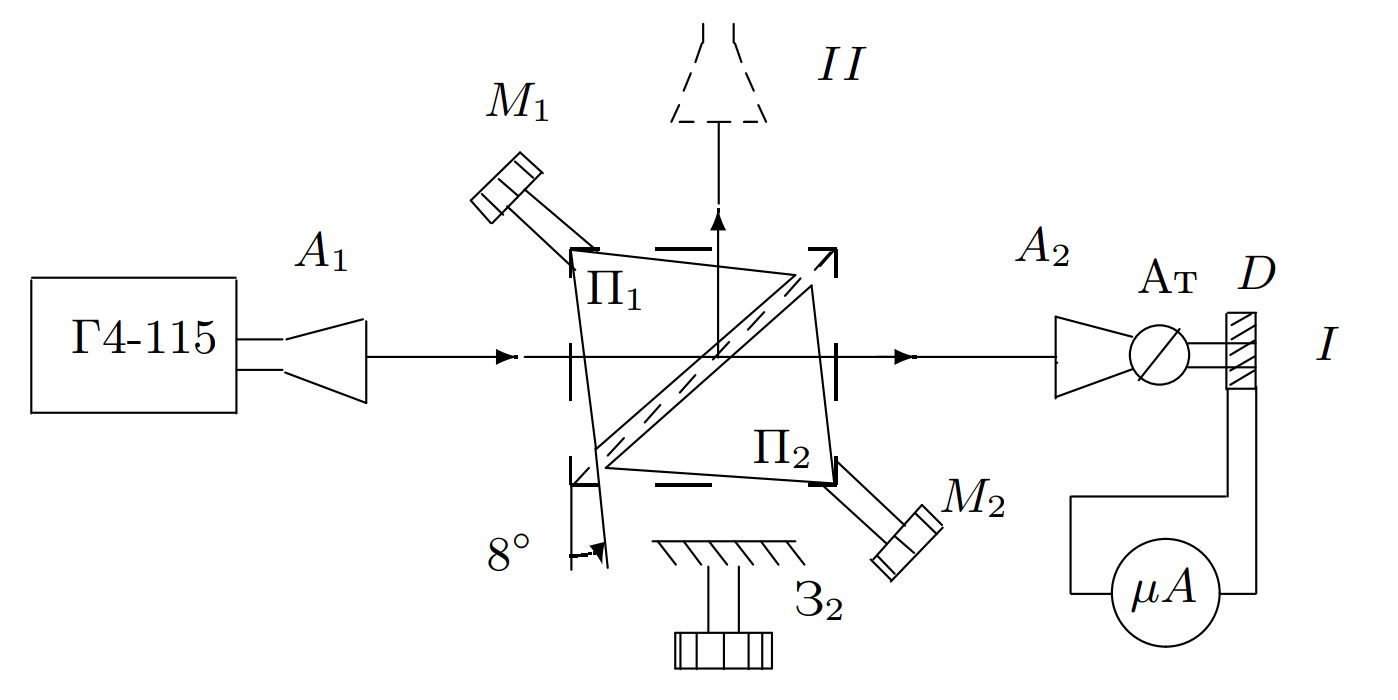
\includegraphics[width=0.8\linewidth]{pics/setup-1.png}
  \caption{Схема установки}
  \label{pic:setup}
\end{figure}
Вторая рупорная антенна $A_2$ служит приёмником радиоволн. Попадая в антенну $A_2$, 
электромагнитная волна распространяется далее по волноводу, аналогичному волноводу 
генератора. Детектор D, расположенный в волноводе, подсоединяется к микроамперметру.
Ток детектора пропорционален интенсивности принимаемого антенной электромагнитного
излучения:
$$\J \propto I$$

\begin{wrapfigure}[7]{r}{0.3\linewidth}
  \vspace{-18mm}
  \begin{center}
    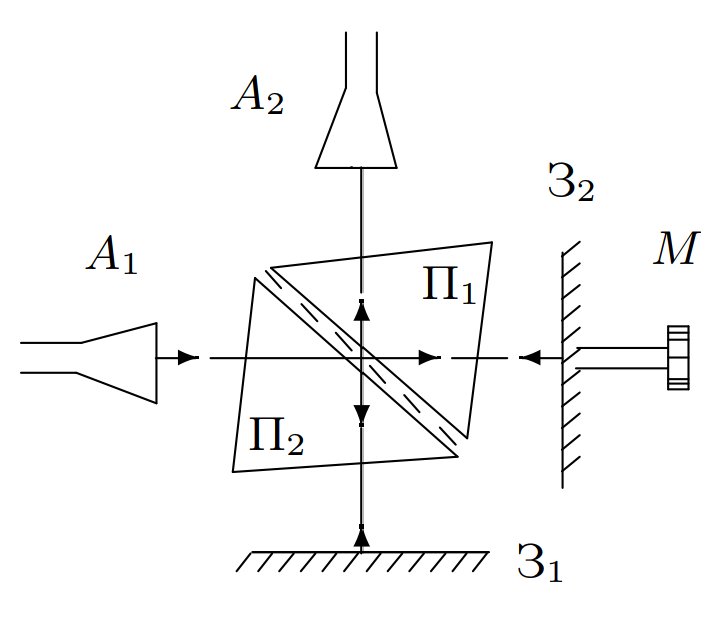
\includegraphics[width=0.90\linewidth]{pics/setup-2.png}
  \end{center}
  \vspace{-8mm}
  \caption{Схема интерферометра Майкельсона}
  \label{pic:interferometer}
\end{wrapfigure}
Аттенюатор Ат позволяет ослаблять сигнал. В положении I антенна A2 принимает сигнал,
прошедший воздушный промежуток, в положении II — сигнал, отражённый от воздушного 
промежутка.

Небольшая реконструкция схемы позволяет смоделировать интерферометр Майкельсона 
(рис. \ref{pic:interferometer}). Воздушный зазор между призмами здесь используется
в качестве делителя волны; зеркало $З_1$ установлено неподвижно, зеркало $З_2$ 
может перемещаться с помощью микрометрического винта M.

\section{Методика измерений и результаты}

\subsection{Часть 1. Коэффициенты прозрачности и отражения.}
Настроим генератор на максимальную выходную мощность. Настройка выполнена на частоту
$f = 36.00\GHz$. Юстировкой установки добьёмся максимального отклика амперметра на сигнал.

При выполнении работы были замечены три особенности установки. Во-первых, имеется существенный
люфт при повороте правого микрометрического винта. Мы будем его компенсировать монотонностью
изменения ширины воздушного промежутка между призмами.

Во-вторых, плоскости призм не остаются строго параллельными. Это видно на начальном этапе работы,
когда воздушный промежуток лишь начинает появляться -- призмы некоторое время продолжаюют 
соприкасаться соответсвующими углами. Кроме того, это вызывает некоторый рост тока
микроамперметра, поэтому регулировка аттенюатора происходила в момент, когда ток максимален.
При этом выставлено значение $\J_\text{max} = 10.0 \uA$. Рост тока из-за непараллельности
при этом составил $\Delta \J = 0.4 \uA$.

В-третьих, генерация происходит с непостоянной мощностью -- при наблюдении показаний без
изменения параметров установки были зафиксированы колебания до $\Delta \J _\text{osc} = 0.3\uA$

Таким образом, примем оценку погрешности измерения тока за $\sigma (\J) = \sqrt{0.4^2 + 0.3^2}\uA
\approx 0.5 \uA$.

Снимем по отдельности (по одинаковым точкам) зависимость тока приёмника при тунеллировании и 
отражении, результаты представлены в \textit{таблице. \ref{table:currents}}.

\begin{table}[H]
  \centering
  \begin{tabular}{|c|c|c|c|}
      \hline
      $I_t,\uA$ & $I_t,\uA$ & $x,\mim$ & $\Delta x,\mim$ \\ \hline
      10.0 & 0.1 & 6.45 & 0.00 \\ \hline
      9.3 & 0.8 & 6.90 & 0.45 \\ \hline
      8.7 & 1.3 & 7.08 & 0.63 \\ \hline
      7.8 & 2.1 & 7.41 & 0.96 \\ \hline
      7.3 & 2.6 & 7.54 & 1.09 \\ \hline
      6.8 & 3.1 & 7.74 & 1.29 \\ \hline
      6.3 & 3.5 & 7.86 & 1.41 \\ \hline
      5.6 & 3.9 & 8.04 & 1.59 \\ \hline
      4.9 & 4.3 & 8.22 & 1.77 \\ \hline
      4.3 & 4.9 & 8.41 & 1.96 \\ \hline
      3.9 & 5.3 & 8.55 & 2.10 \\ \hline
      3.4 & 5.8 & 8.76 & 2.31 \\ \hline
      2.9 & 6.2 & 8.97 & 2.52 \\ \hline
      2.4 & 6.7 & 9.25 & 2.80 \\ \hline
      1.9 & 7.1 & 9.53 & 3.08 \\ \hline
      1.5 & 7.9 & 10.14 & 3.69 \\ \hline
      1.0 & 9.0 & 11.34 & 4.89 \\ \hline
  \end{tabular}
  \caption{Экспериментальные данные: зависимость тока $I_t$ и $I_r$ от смещения $\Delta x$.}
  \label{table:currents}
\end{table}

По полученным данным построим графики зависимостей, а так же их предполагаемую линеаризацию (согласно (\ref{eq:intensity_propto})).
Результаты представлены на \textit{рис. \ref{pic:res_lin} и \ref{pic:res_log}}.

Видно, что сумма $R+T$ несущественно выходит за $1\sigma$-границу 100\% ($\sqrt{5^2 + 5^2}\% \approx 7.1 \%$), что означает что условие 
$R+T = 1$ можно считать выполненным. Пересечение зависимостей происходит при $R=T\approx 0.5$, при этом 
$\Lambda_\text{intersect} = (1.87\pm0.17)\mim$.

На втором графике видно, что в случае интенсивности в отраженном излучении, линеаризация плохо справляется с задачей.
Удовлетворительные результаты получаются в пропущенном излучении~-- угол наклона при этом соответсвует 
$\Lambda_\text{descent} = (2.14\pm 0.14) \mim$.

Тогда примем значение $\Lambda$ за $(2.00 \pm 0.22)\mim$ (усреднение среднего, сложение квадратов отклонений).
\begin{figure}[H]
  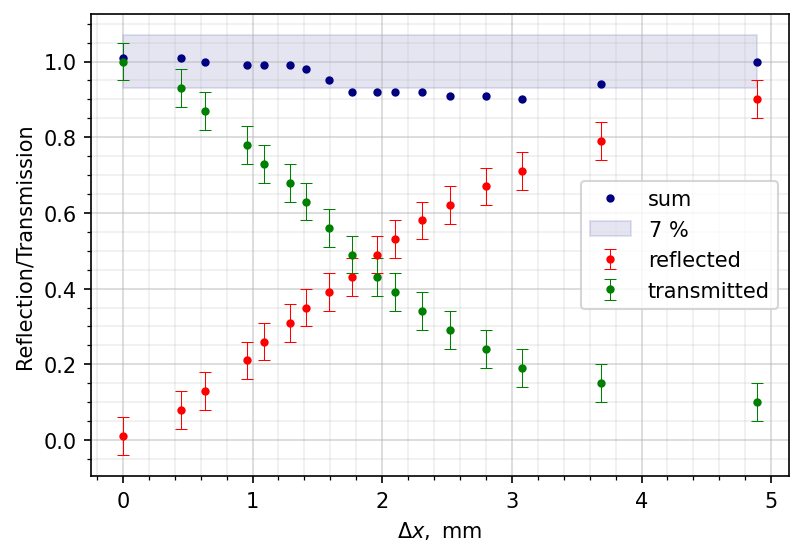
\includegraphics[width=0.8\linewidth]{pics/results-1-linear.png}
  \caption{График зависимости коэффициентов прозрачности и отражения от величины зазора}
  \label{pic:res_lin}
\end{figure}
\begin{figure}[H]
  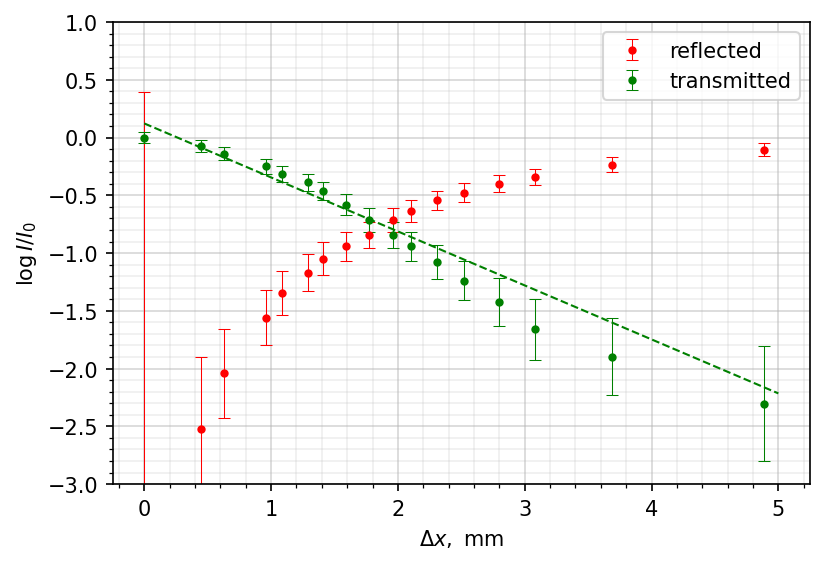
\includegraphics[width=0.8\linewidth]{pics/resluts-2-log.png}
  \caption{Предполагаемая линеаризация зависимости}
  \label{pic:res_log}
\end{figure}

Модифицируем определния $\varkappa, \Lambda$ из теоретической части:
\[\Lambda = \frac{\lambda_\text{возд}}{4\pi\sqrt{n^2 \sin^2 \varphi_1  - 1}}\]

Несмотря на большую погрешность $\Lambda$, близость $n\sin \varphi$ к единице позволяет достаточно точно оценить $n\sin\varphi$:

\[n\sin\varphi = \sqrt{\left( \frac{\lambda_\text{возд}}{4\pi \Lambda} \right)^2 + 1} \approx 1.053,\quad \varepsilon(n\sin \varphi) \approx 1.2\%\]

В таком случае куда больший вклад в погрешность $n$ даст неточность определения угла. Оценим $\sigma{\varphi} = 5^\circ$.
Тогда $n = (1.48\pm0.12)$.

\subsection{Интерферометр Майкельсона}
Настроим установку согласно \textit{рис. \ref{pic:interferometer}}, кроме того так, чтобы $R=T\approx 0.5$.
Снимем зависимость интенсивности в отражённом излучении от сдвига подвижного зеркала. Результат -- на \textit{рис. \ref{pic:interfere}}.
\begin{figure}[H]
  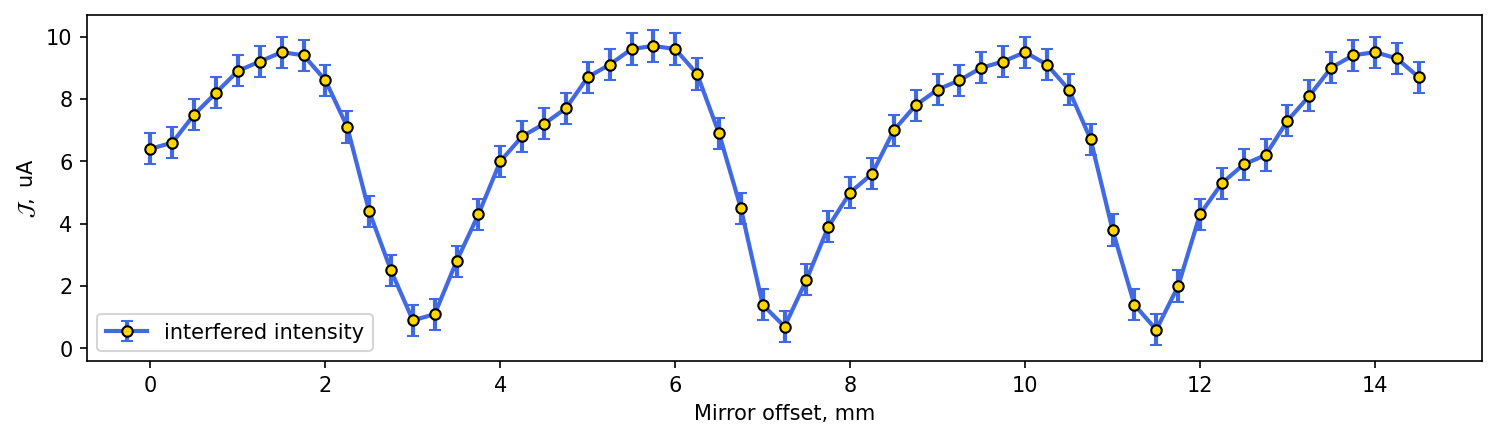
\includegraphics[width=0.8\linewidth]{pics/interfere-raw.png}
  \caption{Зависимость измеренной интенсивности от сдвига зеркала}
  \label{pic:interfere}
\end{figure}
Синусоидальная зависимость здесь, конечно, не выполнена, но очевиден повторяющийся профиль функции.
Попробуем провести анализ следующим образом: разделить данные на 3 <<периода>>
и найти такой сдвиг данных, при которых площадь под максимальной разницей интерполированных по точкам функций была бы минимальна.
Оптимальное решение составляет $\Delta x_{opt} = (4.20\pm0.09)\mim$. Погрешность оценим по изменению оптимизируемой велиичны
так, как будто вся область расширена на одну стандартную ошибку.
Иллюстрация -- на \textit{рис. \ref{pic:optimization}}.
\begin{figure}[H]
  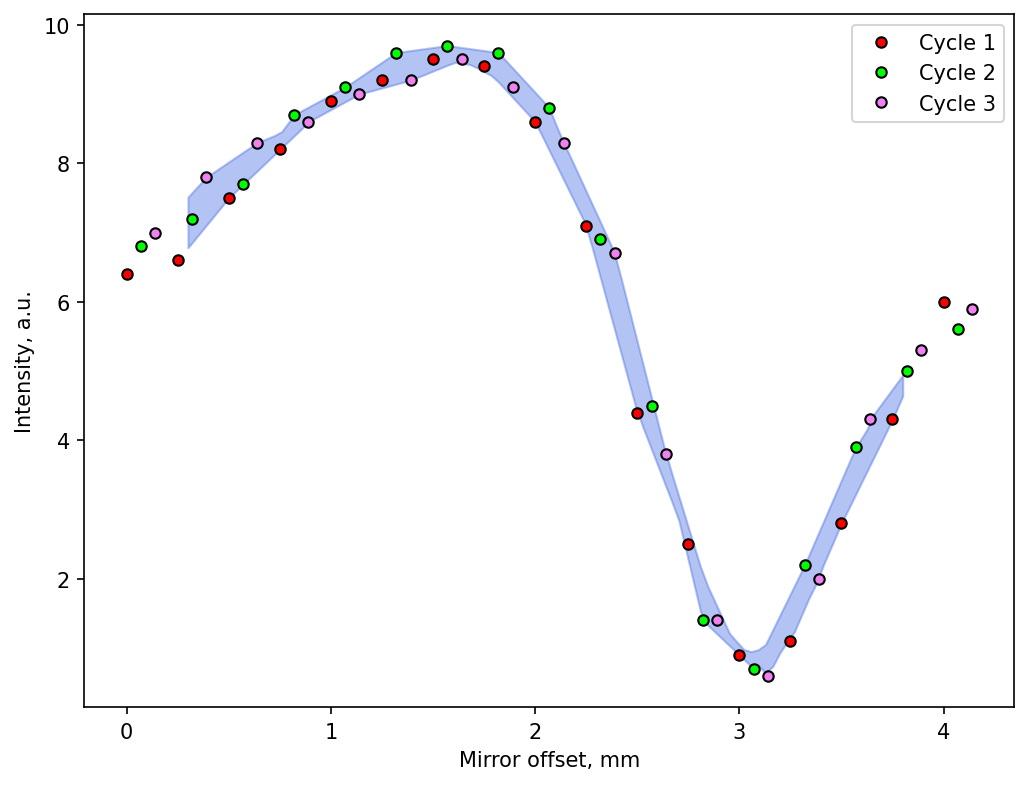
\includegraphics[width=0.65\linewidth]{pics/interfere-offset.png}
  \caption{Оптимизация и нахождение периода}
  \label{pic:optimization}
\end{figure}

То есть длина волны в воздухе составляет $\lambda = 2\cdot\Delta x_{opt} = (8.40\pm0.18) \mim$, при этом от генератора ожидается 
$\lambda_\text{gen} = 8.33 \mim$ -- отличное совпадение.

Зная приблизительное значение показателя преломления $n\sim1.5$ и толщины пластины $h=(6.2\pm0.1)\mim$, понимаем, что изменения 
порядка интерференции не происходит: $(h(n-1)) < \lambda/2$.

Тогда трижды будем ставить и убирать неподвижное зеркало и смотреть, на какое расстояние нужно сдвинуть подвижное, чтобы вернуться
к максимуму интенсивности. Результаты -- в \textit{таблице \ref{table:interferention}}.

\begin{table}[H]
  \begin{tabular}{|l|l|l|}
  \hline
  $l_1, \mim$  &  $l_2, \mim$  & $\Delta l, \mim$     \\ \hline
  1.76  & 3.17  & 1.41 \\ \hline
  10.30 & 11.64 & 1.34 \\ \hline
  6.00  & 7.30  & 1.30 \\ \hline
  \end{tabular}
  \caption{Результаты интерферометрии}
  \label{table:interferention}
\end{table}
Таким образом, $\Delta l = (1.35\pm0.5)\mim$.
Получим тогда $n =  \Delta l \cdot 2 / h + 1 \approx (1.435\pm0.15)$.

\section{Обсуждение результатов и выводы}
В ходе работы были выполнены две части. 
Во-первых, были получены зависимости коэффициента пропускания и отражения при тунеллировании
излучения при ПВО, проверено утверждение $R+T=1$. Тем не менее, одна из зависимостей неудовлетворительно описывается теорией.
Причиной тому может быть дифракция на толстых металлических креплениях призм. Из имеющихся данных была найдена длина затухания
неоднородной волны в зазоре, и, соответсвенно, коэффициент преломления $n = (1.48 \pm 0.12)$. 

Во-вторых, с помощью тунеллирования была проведена интерферометрия Майкельсона. Хорошо совпала совпадение длина волны, полученная
интерферометрией, и полученная с показаний генератора. Также было получено значение коэффициента преломления $n=(1.42\pm 0.02)$.

В ГОСТ 10007-80 указано, что дилектрическая проницаемость фторопласта-4 не зависит от частоты и составляет $(2.0\pm0.1)$, что соответсвует
$n=(1.41\pm0.4)$. Таким образом, полученные результаты согласуются со справочными данными.

\end{document}
